%        File: arfc-pres.tex
%     Created: 2018-12-15 10:00 AM 2018 C
%


%\documentclass[11pt,handout]{beamer}
\documentclass[9pt,handout]{beamer}
\usetheme[white]{Illinois}
%\title[short title]{long title}
\title[Kineticss in Liquid-Fueled Reactors]{Neutron Kinetics and Dynamics in Liquid-Fueled Nuclear Reactors}
%\subtitle[short subtitle]{long subtitle}
\subtitle[Purdue]{Purdue Nuclear Engineering Seminar}
%\author[short name]{long name}
\author[Huff]{Kathryn Huff\\Advanced Reactors and Fuel Cycles Group}
%\date[short date]{long date}
\date[02.20.2019]{February 20, 2019}
%\institution[short name]{long name}
\institute[UIUC]{University of Illinois at Urbana-Champaign}

\usepackage{lmodern}
%\usepackage{bbding}
\usepackage{amsfonts}
\usepackage{amsmath}
\usepackage{xspace}
\usepackage{graphicx}
%\usepackage{caption}  % allows center figures caption
\usepackage{notoccite}
\usepackage{animate}
\usepackage{subfigure}
\usepackage{booktabs} % nice rules for tables
\usepackage{microtype} % if using PDF
\usepackage{bigints}
\newcommand{\units}[1] {\:\text{#1}}%
\newcommand{\SN}{S$_N$}%{S$_\text{N}$}%{$S_N$}%
\DeclareMathOperator{\erf}{erf}
%I need some complimentary error funcitons... 
\DeclareMathOperator{\erfc}{erfc}
%Those icons in the references are terrible looking
\setbeamertemplate{bibliography item}[text]

%%%% Acronym support

\usepackage[acronym,toc]{glossaries}
\include{acros}

\makeglossaries

%try to get rid of header on title page\dots
\makeatletter
    \newenvironment{withoutheadline}{
        \setbeamertemplate{headline}[default]
        \def\beamer@entrycode{\vspace*{-\headheight}}
    }{}
\makeatother

\makeatother
\setbeamertemplate{footline}
{
  \leavevmode%
  \hbox{%
    \rightline{\insertframenumber{} / \inserttotalframenumber\hspace*{1ex}}
  }%
  \vskip0pt%
}
\makeatletter
\begin{document}
%%%%%%%%%%%%%%%%%%%%%%%%%%%%%%%%%%%%%%%%%%%%%%%%%%%%%%%%%%%%%
%% From uw-beamer Here's a handy bit of code to place at 
%% the beginning of your presentation (after \begin{document}):
\newcommand*{\alphabet}{ABCDEFGHIJKLMNOPQRSTUVWXYZabcdefghijklmnopqrstuvwxyz}
\newlength{\highlightheight}
\newlength{\highlightdepth}
\newlength{\highlightmargin}
\setlength{\highlightmargin}{2pt}
\settoheight{\highlightheight}{\alphabet}
\settodepth{\highlightdepth}{\alphabet}
\addtolength{\highlightheight}{\highlightmargin}
\addtolength{\highlightdepth}{\highlightmargin}
\addtolength{\highlightheight}{\highlightdepth}
\newcommand*{\Highlight}{\rlap{\textcolor{HighlightBackground}{\rule[-\highlightdepth]{\linewidth}{\highlightheight}}}}
%%%%%%%%%%%%%%%%%%%%%%%%%%%%%%%%%%%%%%%%%%%%%%%%%%%%%%%%%%%%%
%%--------------------------------%%
\begin{withoutheadline}
\frame{
  \titlepage
}
\end{withoutheadline}

%%--------------------------------%%
\AtBeginSection[]{
\begin{frame}
  \frametitle{Outline}
  \tableofcontents[currentsection]
\end{frame}
}

\section{Introduction}
\subsection{NPRE}
\begin{frame}
        \frametitle{Nuclear, Plasma, and Radiological Engineering}
        BS, MS, and PhD in three degree paths:
        \begin{itemize}
              \item Plasmas and Fusion
              \item Power, Safety and the Environment
              \item Radiological, Medical and Instrument Applications
        \end{itemize}

\end{frame}
\begin{frame}
        \frametitle{Nuclear, Plasma, and Radiological Engineering}
               \begin{figure}[t]
                \vspace*{-0.1in}
                \includegraphics[width=\textwidth]{./images/npre-fac1.png}
                \includegraphics[width=0.33\textwidth]{./images/npre-fac2.png}
               \end{figure}            
        
\end{frame}


\begin{frame}
  \frametitle{NPRE Growth}
Enrollment
        \begin{itemize}
                \item 123 Undergraduates - NPRE
                \item 95 Graduate Students - NPRE
                \item 30 Master of Energy Systems Students
        \end{itemize}
               \begin{figure}[t]
                \vspace*{-0.1in}
                \includegraphics[width=\textwidth]{./images/npre_growth.png}
                       \caption{Current undergraduate and graduate students.}
               \end{figure}            
\end{frame}

\subsection{About ARFC}
\begin{frame}
  \frametitle{Advanced Reactors and Fuel Cycles group (PI: Kathryn Huff)}
               \begin{figure}[t]
                \vspace*{-0.1in}
                \includegraphics[height=0.71\textwidth]{./images/arfc1.png}
               \end{figure}            
\end{frame}

\begin{frame}
  \frametitle{Insights at Disparate Scales}
               \begin{figure}[t]
                \vspace*{-0.1in}
			\hspace*{-0.35in}
                \includegraphics[height=0.5\textwidth]{./images/synergy.png}
               \end{figure}            
\end{frame}

\subsection{Fission basics}
\begin{frame}
  \frametitle{Nuclear Fission Reaction}
               \begin{figure}[t]
                \vspace*{-0.1in}
			\hspace*{-0.35in}
                \includegraphics[height=0.25\textwidth]{./images/800px-Fission.png}
               \end{figure}            
\end{frame}

\begin{frame}
  \frametitle{Nuclear Fission Chain Reaction}
               \begin{figure}[t]
                \vspace*{-0.1in}
			\hspace*{-0.35in}
                \includegraphics[height=0.7\textwidth]{./images/715px-Chainreaction.png}
               \end{figure}            
\end{frame}

\begin{frame}
  \frametitle{Nuclear Power Plant}
  \animategraphics[width=\textwidth,autoplay,loop]{6}{./images/gif/frame-}{0}{23}
\end{frame}

\subsection{Motivation}
\begin{frame}
  \frametitle{Why Molten Salt Reactors?}
                  \vspace*{-0.1in}
              \begin{block}{Main advantages of liquid-fueled \glspl{MSR} \cite{elsheikh_safety_2013}}
               \begin{enumerate}
                \item High coolant temperature (600-750$^{\circ}$C).
                \item Various fuels can be used ($^{235}$U, $^{233}$U, Thorium, U/Pu).
                \item Increased inherent safety.
                \item High fuel utilization $\Rightarrow$ less nuclear waste generated.
                \item Online reprocessing and refueling.
               \end{enumerate}
               \end{block}
                  \vspace*{-0.1in}               
               \begin{block}{Main advantages of \gls{MSBR} \cite{robertson_conceptual_1971}}
               \begin{enumerate}
                \item Produces more fissile material than it consumes (breeding ratio 1.06).
                \item Thorium cycle limits plutonium and minor actinides.
                \item Could transmute spent fuel from existing \gls{NPP}.
               \end{enumerate}
               \end{block}

\end{frame}

\begin{frame}
  \frametitle{Challenges in simulation \gls{MSR}}
                  \vspace*{-0.05in}
               \begin{enumerate}
                \item Contemporary burnup codes cannot treat fuel movement.
                \item Neutron precursor location is hard to estimate.
                \item Operational and safety parameters change during reactor operation.
                \item Power generation strongly depends on fuel temperature and vica versa.
               \end{enumerate}

           \begin{figure}[t]
                \vspace*{-0.3in}
			\hspace*{-0.2in}
                \includegraphics[height=0.5\textwidth]{./images/coupled_physics.png}
		\vspace*{-0.05in}
		\caption{Multiphysics simulation scheme for \gls{MSR} (Courtesy of Manuele Aufiero,2012).}
     	 \end{figure}               
\end{frame}

\begin{frame}
  \frametitle{Research objectives}
                  \vspace*{-0.1in}
              \begin{block}{Goal \#1: Tool for online reprocessing depletion simulation (SaltProc)\cite{rykhlevskii_saltproc}}
               \begin{enumerate}
                \item Create high-fidelity full-core 3-D model of MSBR without any approximations using the continuous-energy SERPENT 2 Monte Carlo physics software \cite{leppanen_serpent_2012}.
                \item Develop online reprocessing simulation code, SaltProc, which expands the capability of SERPENT for simulation liquid-fueled \gls{MSR} operation.
                \item Analyse \gls{MSBR} neutronics and fuel cycle to find the equilibrium core composition and core depletion.
                \item Compare predicted operational and safety parameters of the \gls{MSBR} at both the initial and equilibrium states.
               \end{enumerate}
               \end{block}

              \begin{block}{Goal \#2: Tool for multiphysics simulation of \gls{MSR} (Moltres)\cite{lindsay_introduction_2018}}
               \begin{enumerate}
                \item Demonstrate steady-state coupling of neutron fluxes, precursors, and temperature for thermal \gls{MSR} design.
                \item Implement advective movement of delayed neutron precursors.
                \item Demonstrate capabilities with 2D axisymmetric and 3D structured/unstructured mesh.
               \end{enumerate}
               \end{block}


              
\end{frame}

\section{Point Kinetics \& TH Coupling}
\subsection{Point and Multi-point Kinetics}
\begin{frame}
        \frametitle{PyRK: Python for Reactor Kinetics}

               \begin{figure}[t]
                \vspace*{-0.1in}
                \includegraphics[height=0.5\textheight]{./images/pyrk.png}
                       \caption{Special purpose reactor kinetics python tool
                       (https://github.com/pyrk/pyrk) \cite{huff_pyrk:_2015}. 
                       Research software for simple PRKE: \emph{caveat emptor.}}
               \end{figure}

               \begin{itemize}
                       \item Multiple precursor groups ($j$ groups)
                       \item Multiple decay heat groups ($k$ groups)
                       \item Lumped Parameter thermal hydraulics model
                       \item Optional 1-D conduction in pebble fuel compacts
                       \item Object-oriented, geometry and material agnostic framework
               \end{itemize}
\end{frame}


%------------------------------------------------------------------------------------
\begin{frame}
        \frametitle{Point Reactor Kinetics}
        \begin{align}
    p &= \mbox{ reactor power }\\
    \rho(t,&T_{fuel},T_{cool},T_{mod}, T_{refl}) = \mbox{ reactivity}\\
    \beta &= \mbox{ fraction of neutrons that are delayed}\\
    \beta_j &= \mbox{ fraction of delayed neutrons from precursor group j}\\
    \zeta_j &= \mbox{ concentration of precursors of group j}\\
    \lambda_{d,j} &= \mbox{ decay constant of precursor group j}\\
    \Lambda &= \mbox{ mean generation time }\\
    \omega_k &= \mbox{ decay heat from FP group k}\\
    \kappa_k &= \mbox{ heat per fission for decay FP group k}\\
    \lambda_{FP,k} &= \mbox{ decay constant for decay FP group k}\\
    T_i &= \mbox{ temperature of component i}
\end{align}

\end{frame}

%------------------------------------------------------------------------------------
\begin{frame}
\frametitle{Point Reactor Kinetics}
\begin{equation}
\frac{d}{dt}\left[
    \begin{array}{c}
      p\\
      \zeta_1\\
      .\\
      \zeta_j\\
      .\\
      \zeta_J\\
      \omega_1\\
      .\\
      \omega_k\\
      .\\
      \omega_K\\
      T_{i}\\
      .\\
      T_{I}\\
    \end{array}
    \right]
    =
    \left[
      \begin{array}{ c }
        \frac{\rho(t,T_{i},\cdots)-\beta}{\Lambda}p +
        \displaystyle\sum^{j=J}_{j=1}\lambda_{d,j}\zeta_j\\
        \frac{\beta_1}{\Lambda} p - \lambda_{d,1}\zeta_1\\
        .\\
        \frac{\beta_j}{\Lambda}p-\lambda_{d,j}\zeta_j\\
        .\\
        \frac{\beta_J}{\Lambda}p-\lambda_{d,J}\zeta_J\\
        \kappa_1p - \lambda_{FP,1}\omega_1\\
        .\\
        \kappa_kp - \lambda_{FP,k}\omega_k\\
        .\\
        \kappa_{k p} - \lambda_{FP,k}\omega_{k}\\
        f_{i}(p, C_{p,i}, T_{i}, \cdots)\\
        .\\
        f_{I}(p, C_{p,I}, T_{I}, \cdots)\\
      \end{array}
      \right]
\end{equation}
\end{frame}

%------------------------------------------------------------------------------------
\begin{frame}
        \frametitle{Lumped Parameter Heat Transfer}

The heat flow out of body $i$ is the sum of surface heat flow by conduction,
convection, radiation, and other mechanisms to each adjacent body, $j$:
\begin{align}
Q &= Q_i + \sum_j Q_{ij}\\
  &=Q_i +  \sum_j\frac{T_{i} - T_{j}}{R_{th,ij}}\\
\dot{Q} &= \mbox{total heat flow out of body i }[J\cdot s^{-1}]\\
Q_i &= \mbox{other heat transfer, a constant }[J\cdot s^{-1}]\\
T_i &= \mbox{temperature of body i }[K]\\
T_j &= \mbox{temperature of body j }[K]\\
j &= \mbox{adjacent bodies }[-]\\
R_{th} &= \mbox{thermal resistence of the component }[K \cdot s \cdot J^{-1}].
\end{align}
\end{frame}

%------------------------------------------------------------------------------------
\begin{frame}
        \frametitle{PB-FHR Example}

               \begin{figure}[t]
                \vspace*{-0.1in}
                       \includegraphics[height=0.5\textwidth]{./images/pbfhr-fuel-movement.png}
                       \caption{The pebble fuel can be assumed approximately 
                       stationary, as their movement is not comparable to the 
                       longest precursor decay times.}
               \end{figure}

\end{frame}


%------------------------------------------------------------------------------------
\begin{frame}
        \frametitle{Point Reactor Kinetics}

               \begin{figure}[t]
                \vspace*{-0.1in}
                       \includegraphics[height=0.5\textwidth]{./images/pbfhr-total-reactivity.png}
                       \caption{Total reactivity during ramped reactivity 
                       insertion as a function of inserted reactivity
                       \cite{wang_coupled_2016}.}
               \end{figure}

\end{frame}



%------------------------------------------------------------------------------------
\begin{frame}
        \frametitle{PB-FHR Example}

               \begin{figure}[t]
                \vspace*{-0.1in}
                       \hspace*{-0.3in}
                       \includegraphics[height=0.3\textwidth]{./images/pbfhr-fuel-temp.png}
                       \includegraphics[height=0.3\textwidth]{./images/pbfhr-avg-pow.png}
                       \includegraphics[height=0.3\textwidth]{./images/pbfhr-coolant-temp.png}
                       \caption{Average fuel temperature (left) and average 
                       normalized core power (right) during a ramp reactivity 
                       insertion in the PB-FHR \cite{wang_coupled_2016}.}
               \end{figure}

\end{frame}


%------------------------------------------------------------------------------------
\begin{frame}
        \frametitle{Point Reactor Kinetics}

               \begin{figure}[t]
                \vspace*{-0.1in}
                       \includegraphics[height=0.5\textwidth]{./images/pbfhr-multi-single-point.png}
                       \caption{Fuel temperature rise following 1\$ ramp 
                       reactivity insertion, calculated with multipoint and 
                       single point kinetics in PyRK \cite{wang_coupled_2016}.}
               \end{figure}

\end{frame}

\section{Spatial Kinetics \& TH Coupling with Precursor Advection}
\begin{frame}
  \frametitle{Moderator element geometry (Zone I)}
    \begin{figure}[t]
                \vspace*{-0.2in}
                   \hspace*{-0.37in}
                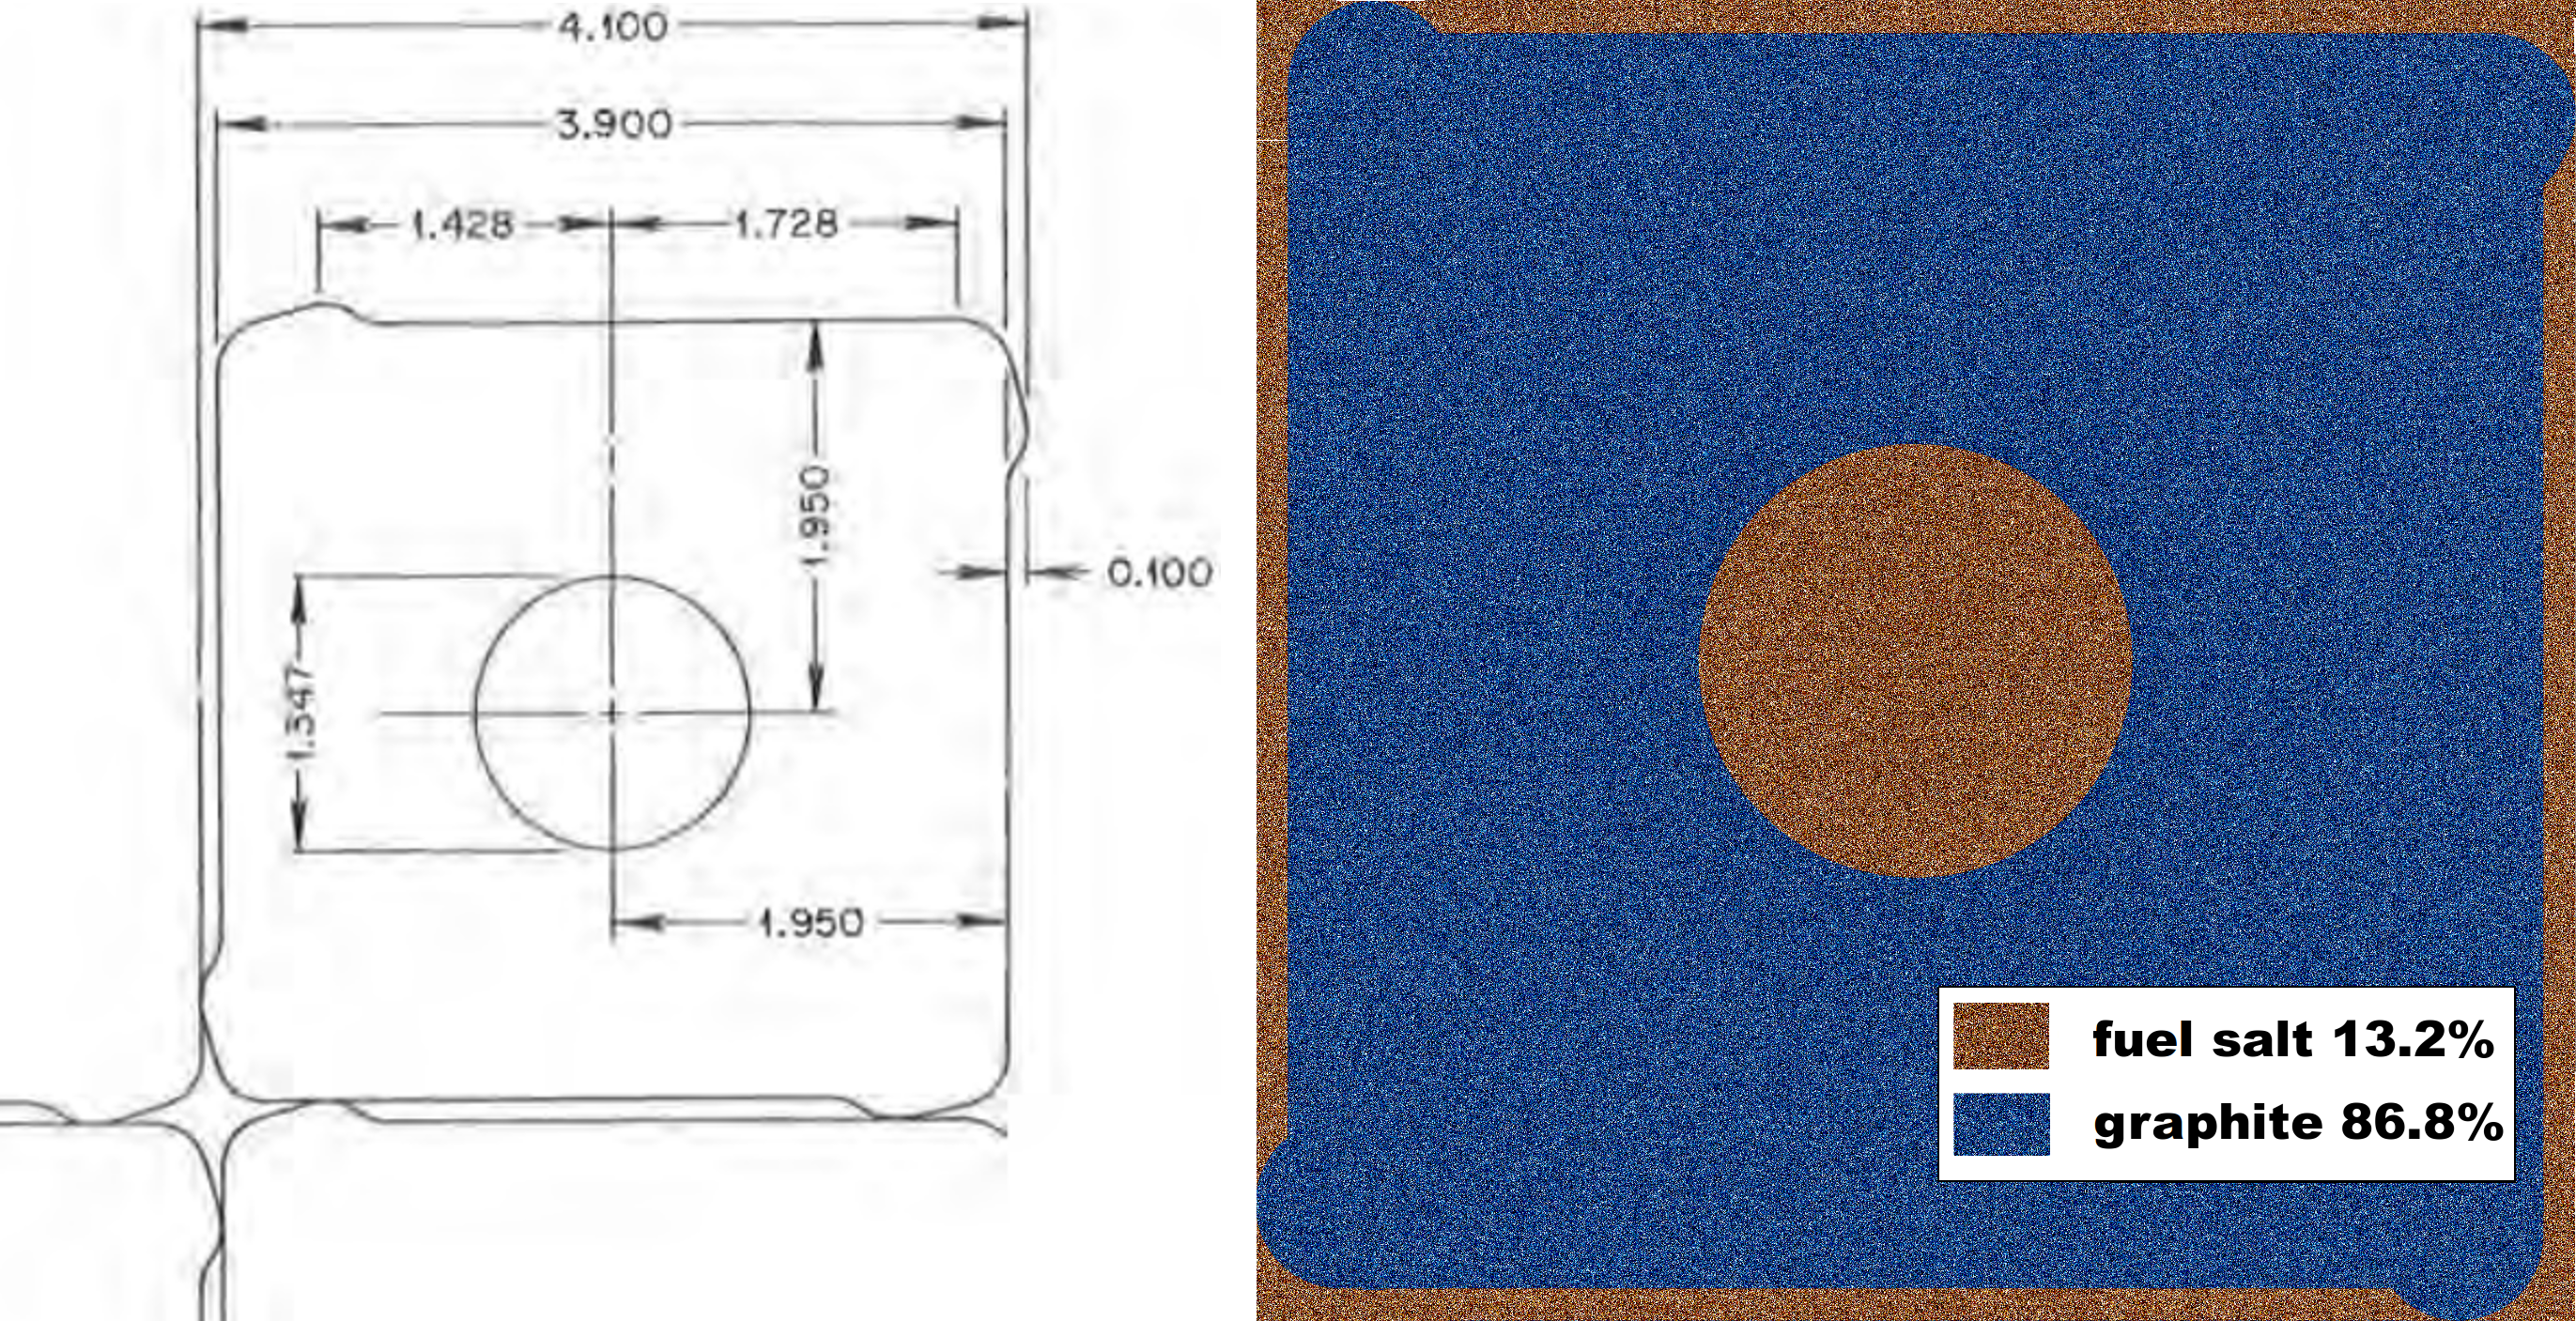
\includegraphics[height=0.60\textwidth]{./images/zone_I_mesh.png}
                \vspace*{-0.05in}
                \caption{Molten Salt Breeder Reactor Zone I unit cell geometry from the reference \cite{robertson_conceptual_1971} (left) and SERPENT 2 (right).}
      \end{figure}
     
\end{frame}

\begin{frame}
  \frametitle{Full-core SERPENT model of \gls{MSBR}}
    \begin{figure}[t]
                \vspace*{-0.2in}
                   \hspace*{-0.39in}
                \includegraphics[height=0.6\textwidth]{./images/geometry_main_views.png}
                \caption{Plan (left) and elevation (right) view of MSBR model.}
      \end{figure}
     
\end{frame}

\begin{frame}
  \frametitle{Core Zone II}
  \begin{figure}[t]
     \vspace{-0.25in}
       \hspace*{-0.43in}
       \includegraphics[height=0.77\textheight]{./images/reflector_and_elements.png}
            \caption{Detailed plan view of graphite reflector and moderator elements.}
  \end{figure}
           \vspace{-0.1in}
\end{frame}

\begin{frame}
\frametitle{Online reprocessing method}
  \begin{columns}
    \column[t]{6cm}
	\begin{figure}[t]
                \vspace*{-0.35in}
			\hspace{-0.3in}
                 \includegraphics[height=\textwidth]{./images/saltproc_flowchart.pdf}
                \vspace*{-0.05in}
                \caption{Flow chart for the SaltProc.}
      \end{figure}

    \column[t]{6cm}
             \begin{block}{SaltProc capabilities}
               \begin{itemize}             
               \item Remove specific isotopes from the core with specific parameters (reprocessing interval, mass rate, removal efficiency)
               \item Add specific isotopes into the core
               \item Maintain constant number density of specific isotope in the core
	       \item Time-dependent material feed and removal rates
	       \item Store stream vectors in an HDF5 database for further analysis or plots
	       \item Generic geometry: an infinite medium, a unit cell, a multi-zone simplified assembly, or a full-core
               \end{itemize}
               \end{block}
  \end{columns}
\end{frame}

\begin{frame}
  \frametitle{Online reprocessing method}
     \begin{figure}[t]
                \vspace*{-0.1in}
                  % \hspace*{-0.37in}
                \includegraphics[height=0.45\textwidth]{./images/pa_isolation.png}
                \vspace*{-0.07in}
                \caption{Protactinium isolation with uranium removal by fluorination \cite{robertson_conceptual_1971}.}
      \end{figure}
                      \vspace*{-0.17in}
             \begin{block}{Online reprocessing approach}
               \begin{itemize}             
               \item Continuously removes all poisons, noble metals, and gases.
               \item $^{233}$Pa is continuously removed from the fuel salt into a decay tank.
               \end{itemize}
               \end{block}
               \vspace{-0.05in}
$\qquad\qquad\qquad\qquad^{232}_{90}$Th+$^1_0$n$\rightarrow^{233}_{90}$Th$\xrightarrow[\text{22.3 min}]{\beta^-}$ $^{233}_{91}$Pa$\xrightarrow[\text{26.967 d}]{\beta^-}$ $^{233}_{92}$U
\end{frame}

\begin{frame}
  \frametitle{MOOSE Framework}
  \begin{columns}
    \column[t]{6cm}
  \begin{figure}[t]
     \vspace{-0.25in}
       \hspace*{-0.25in}
       \includegraphics[height=0.65\textheight]{./images/moose.png}
            \caption{Multi-physics Object-Oriented Simulation Environment (MOOSE).}
  \end{figure}
	\column[t]{6cm}
               \begin{itemize}      
	       \item Fully-coupled, fully-implicit multiphysics solver      
               \item MOOSE interfaces with libMesh to discretize simulation volume into finite elements
               \item Residuals and Jacobians handed off to PetSc which handles solution of resulting non-linear system of algebraic equations
	       \item Automatically parallel (largest runs \textgreater 100,000 CPU cores!)
	       \item Built-in mesh adaptivity
	       \item Intuitive parallel multiscale solves
               \end{itemize}

  \end{columns}
\end{frame}


\begin{frame}
  \frametitle{Effective multiplication factor for full-core \gls{MSBR} model }
    \begin{columns}
    \column[t]{7cm}
   \vspace{-0.35in}
  \begin{figure}[t]
   \hspace*{-0.2in}
   \includegraphics[height=0.75\textheight]{./images/keff.png}
   \vspace{-0.05in}
   \caption{$k_{eff}$ during a 20 years depletion simulation.}
    \end{figure}

    \column[t]{4.5cm}
       \begin{itemize}
	        \item Strong absorbers ($^{233}$Th,$^{234}$U) accumulating in the core
   		\item Fissile materials other than $^{233}$U are bred into the core ($^{235}$U, $^{239}$Pu)
   		\item The multiplication factor stabilizes after approximately 6 years
       \end{itemize}
     \end{columns}
\end{frame}

\begin{frame}
  \frametitle{Power and breeding distribution}
    \begin{columns}
    \column[t]{6cm}
  \begin{figure}[t]
   \vspace{-0.25in}
   \hspace*{-0.15in}
   \includegraphics[height=0.6\textheight]{./images/power_distribution.png}
   \vspace{-0.1in}
   \caption{Normalized power density}
    \end{figure}

    \column[t]{6cm}
  \begin{figure}[t]
   \vspace{-0.25in}
	\hspace*{-0.05in}
   \includegraphics[height=0.6\textheight]{./images/breeding_distribution.png}
   \vspace{-0.1in}
   \caption{$^{232}$Th neutron capture reaction rate normalized by total flux}
    \end{figure}

     \end{columns}
\end{frame}

\begin{frame}
  \frametitle{$^{232}$Th refill rate}
    \begin{columns}
    \column[t]{7cm}
   \vspace{-0.35in}
  \begin{figure}[t]
   \hspace*{-0.2in}
   \includegraphics[height=0.75\textheight]{./images/Th_refill_rate.png}
   \vspace{-0.05in}
   \caption{$^{232}$Th feed rate over 20 years of \gls{MSBR} operation}
    \end{figure}

    \column[t]{4.5cm}
       \begin{itemize}
	        \item Fluctuation due to batch-wise removal of strong absorbers
   		\item Feed rate varies due to neutron energy spectrum evolution
   		\item $^{232}$Th consumption is 100 g/GWh$_e$
       \end{itemize}
     \end{columns}
\end{frame}

\begin{frame}
  \frametitle{Multiphysics simulation results (2D)}
  \begin{figure}
   \vspace{-0.05in}
   \hspace*{-0.15in}
   \includegraphics[height=0.85\textheight]{./images/moltres_flux.png}
   \vspace{-0.1in}
   \caption{Fast ($\phi_1$) and thermal ($\phi_2$) neutron flux obtained using Moltres 			\cite{lindsay_introduction_2018}.}
    \end{figure}
\end{frame}

\begin{frame}
  \frametitle{Multiphysics simulation results (2D) (2)}
  \begin{figure}[t]
   \vspace{-0.05in}
   \hspace*{-0.15in}
   \includegraphics[height=0.85\textheight]{./images/moltres_temp.png}
   \vspace{-0.1in}
   \caption{Temperature in channel obtained using Moltres \cite{lindsay_introduction_2018}.}
    \end{figure}

\end{frame}

\begin{frame}
  \frametitle{Multiphysics simulation results (3D)}
  \begin{figure}[t]
   \vspace{-0.1in}
   \hspace*{-0.45in}
   \includegraphics[height=0.75\textheight]{./images/moltres_3D.png}
   \caption{Cuboidal \gls{MSR} steady-state temperature and fast neutron flux \cite{ridley_moltres_2017}.}
    \end{figure}

\end{frame}

\begin{frame}
  \frametitle{MOOSE Framework}
  \begin{columns}
    \column[t]{6cm}
  \begin{figure}[t]
     \vspace{-0.25in}
       \hspace*{-0.25in}
       \includegraphics[height=0.65\textheight]{./images/moose.png}
            \caption{Multi-physics Object-Oriented Simulation Environment (MOOSE).}
  \end{figure}
	\column[t]{6cm}
               \begin{itemize}
	       \item Fully-coupled, fully-implicit multiphysics solver
               \item MOOSE interfaces with libMesh to discretize simulation volume into finite elements
               \item Residuals and Jacobians handed off to PetSc which handles solution of resulting non-linear system of algebraic equations
	       \item Automatically parallel (largest runs \textgreater 100,000 CPU cores!)
	       \item Built-in mesh adaptivity
	       \item Intuitive parallel multiscale solves
               \end{itemize}

  \end{columns}
\end{frame}

\begin{frame}
        \frametitle{Moltres (Coupling in MOOSE)}
  \begin{figure}
   \vspace{-0.05in}
   \hspace*{-0.15in}
   \includegraphics[width=1.1\textwidth]{./images/moltres-moose-diag.png}
    \end{figure}
\end{frame}

\begin{frame}
        \frametitle{Inro to Moltres}
        \begin{itemize}  
                \item Fluid-fuelled, molten salt reactors
                \item Multi-group diffusion (arbitrary groups)
                \item Advective movement of delayed neutron precursors
                \item Navier-Stokes thermal hydraulics
                \item 3D unstructured
                \item 2D axisymmetric
                \item 3D structured 
                \item Initial developer: Alexander Lindsay
        \end{itemize}
\end{frame}

\begin{frame}
        \frametitle{Acquiring Moltres}
             \texttt{git clone https://github.com/arfc/moltres}\\
        \texttt{cd moltres}\\
        \texttt{git submodule init}\\
        \texttt{git submodule update}\\
\end{frame}

\begin{frame}
        \frametitle{Diffusion in Moltres}
        \footnotesize{
        \begin{align}
        \frac{1}{v_g}\frac{\partial \phi_g}{\partial t} &- \nabla \cdot D_g
        \nabla \phi_g + \Sigma_g^r \phi_g =\\
                &\sum_{g \ne g'}^G \Sigma_{g'\rightarrow g}^s \phi_{g'} + \chi_g^p \sum_{g' = 1}^G (1 -
        \beta) \nu \Sigma_{g'}^f \phi_{g'} + \chi_g^d \sum_i^I \lambda_i C_i
        \end{align}}
\begin{columns}
    \begin{column}{0.48\textwidth}
        \footnotesize{
        \begin{align*}
                v_g &= \mbox{speed of neutrons in group g} \\
                \phi_g &= \mbox{flux of neutrons in group g} \\
                t &= \mbox{time} \\
                D_g &= \mbox{Diffusion coefficient for neutrons in group g} \\
                \Sigma_g^r &= \mbox{macroscopic cross-section for}\\
                &\mbox{removal of neutrons from group g} \\
                \Sigma_{g'\rightarrow g}^s &= \mbox{macroscopic cross-section 
                of}\\
                &\mbox{  scattering from g' to g} \\
                \chi_g^p &= \mbox{prompt fission spectrum, neutrons in group g} \\
        \end{align*}}
    \end{column}
    \begin{column}{0.48\textwidth}
        %Content
        \footnotesize{
        \begin{align*}
                G &= \mbox{number of discrete groups, g} \\
                \nu &= \mbox{neutrons produced per fission} \\
                \Sigma_g^f &= \mbox{macroscopic fission cross section}\\
                &\mbox{ due to neutrons in group g} \\
                \chi_g^d &= \mbox{delayed neutrons in group g} \\
                I &= \mbox{ delayed neutron precursor groups} \\
                \beta &= \mbox{delayed neutron fraction}\\
                \lambda_i &= \mbox{average decay constant}\\
                &\mbox{of delayed neutron precursors in group i} \\
                C_i &= \mbox{concentration of delayed neutron}\\
                &\mbox{precursors in precursor group i}\\.
        \end{align*}}
    \end{column}
\end{columns}
\end{frame}

\begin{frame}
        \frametitle{Moltres Delayed Neutrons}
        \begin{align}
        \frac{\partial C_i}{\partial t} &= \sum_{g'= 1}^G \beta_i \nu
        \Sigma_{g'}^f \phi_{g'} - \lambda_i C_i - \frac{\partial}{\partial z} u
        C_i \label{eq:precursors}
\end{align}

        \begin{align*}
                G &= \mbox{number of discrete groups, g} \\
                I &= \mbox{ delayed neutron precursor groups} \\
                C_i &= \mbox{concentration of delayed neutron}\\
                &\mbox{precursors in precursor group i}\\.
                u &= \mbox{vertical fluid velocity}\\
                \lambda_i &= \mbox{average decay constant}\\
                &\mbox{of delayed neutron precursors in group i} \\
                \beta &= \mbox{fraction of delayed neutron}\\
                &\mbox{precursors in group i} \\
        \end{align*}
\end{frame}


\begin{frame}
        \frametitle{Moltres Fuel Temperature}
\begin{align}
        \rho_fc_{p,f}\frac{\partial T_f}{\partial t} &+ \nabla\cdot\left(\rho_f
        c_{p,f} \vec{u}\cdot T_f -k_f\nabla T_f\right) =  Q_f
\end{align}
\begin{align}
  \rho_f &= \mbox{density of fuel salt}\\
  c_{p,f} &= \mbox{specific heat capacity of fuel salt}\\
  T_f &= \mbox{temperature of fuel salt}\\
  \vec{u} &= \mbox{velocity of fuel salt}\\
  k_f &= \mbox{thermal conductivity of fuel salt}\\
  Q_f &= \mbox{source term} = \sum_{g=1}^G \epsilon_{f,g}\Sigma_{f,g}\phi_g
\end{align}
\end{frame}


\begin{frame}
        \frametitle{Moltres Moderator Temperature}
\begin{align}
        \rho_gc_{p,g}\frac{\partial T_g}{\partial t} &+
        \nabla\cdot\left(-k_g\nabla T_g\right) =  Q_g\\
\end{align}
\begin{align}
  \rho_g &= \mbox{density of graphite moderator}\\
  c_{p,g} &= \mbox{specific heat capacity of graphite moderator}\\
  T_g &= \mbox{temperature of graphite moderator}\\
  k_g &= \mbox{thermal conductivity of graphite moderator}\\
  Q_g &= \mbox{source term in graphite moderator}\\
\end{align}

\end{frame}


\begin{frame}
        \frametitle{Moltres MSRE Simulation}
  \begin{figure}
   \vspace{-0.05in}
   \includegraphics[height=0.85\textheight]{./images/msre.png}
    \end{figure}
\end{frame}


\begin{frame}
        \frametitle{Moltres MSRE Simulation}
  \begin{figure}
   \vspace{-0.05in}
   \includegraphics[width=1.2\textwidth]{./images/moltres-input.png}
          \caption{Data used in \cite{lindsay_introduction_2018}.}
    \end{figure}
\end{frame}

\begin{frame}
        \frametitle{Moltres MSRE Simulation}
  \begin{figure}
   \vspace{-0.05in}
   \includegraphics[width=0.85\textwidth]{./images/moltres-composition.png}
          \caption{Data used in \cite{lindsay_introduction_2018}.}
    \end{figure}
\end{frame}


\begin{frame}
        \frametitle{Moltres (coupling in MOOSE)}
  \begin{figure}
   \vspace{-0.05in}
   \includegraphics[height=0.85\textheight]{./images/lindsay_msre_moose.png}
    \end{figure}
\end{frame}



\begin{frame}
        \frametitle{Moltres Precursor Drift}
  \begin{figure}
   \vspace{-0.1in}
   \includegraphics[width=0.28\textwidth]{./images/auto_diff_rho_pre1.eps}
   \includegraphics[width=0.28\textwidth]{./images/auto_diff_rho_pre2.eps}
   \includegraphics[width=0.28\textwidth]{./images/auto_diff_rho_pre3.eps}
   \includegraphics[width=0.28\textwidth]{./images/auto_diff_rho_pre4.eps}
   \includegraphics[width=0.28\textwidth]{./images/auto_diff_rho_pre5.eps}
   \includegraphics[width=0.28\textwidth]{./images/auto_diff_rho_pre6.eps}
    \end{figure}
\end{frame}



\begin{frame}
        \frametitle{Moltres MSRE Comparison}
  \begin{figure}
   \vspace{-0.05in}
   \includegraphics[height=0.85\textheight]{./images/moltres-axial.png}
    \end{figure}
\end{frame}


\begin{frame}
        \frametitle{Moltres MSRE Comparison}
  \begin{figure}
   \vspace{-0.05in}
   \includegraphics[height=0.85\textheight]{./images/moltres-axisym-flux.png}
    \end{figure}
\end{frame}


\begin{frame}
        \frametitle{Moltres MSRE Comparison}
  \begin{figure}
   \vspace{-0.05in}
   \includegraphics[height=0.85\textheight]{./images/moltres-axial-flux.png}
    \end{figure}
\end{frame}


\begin{frame}
  \frametitle{Multiphysics simulation results (3D)}
  \begin{figure}[t]
   \vspace{-0.1in}
   \hspace*{-0.45in}
   \includegraphics[height=0.75\textheight]{./images/moltres_3D.png}
   \caption{Cuboidal \gls{MSR} steady-state temperature and fast neutron flux 
          tests by Gavin Ridley.} 
    \end{figure}

\end{frame}

\begin{frame}
    \frametitle{Conclusion}
    Cyclus is a performant, expanding fuel cycle simulator that holds promise for future applications. It demonstrated its capability to:
    \begin{itemize}
        \item `Predict the past'
        \item Model dynamic transition scenarios
        \item Perform sensitivity studies
        \item Visualize important, dynamic fuel cycle metrics
    \end{itemize}
\end{frame}

\begin{frame}
    \frametitle{Future Work Ongoing}
    \texttt{Cycamore} is adequate for rough analyses, but more accurate
    modules or additional tools would increase analysis fidelity
    \begin{itemize}
        \item Dynamic archetype parameters (e.g. \texttt{refuel\_time}
                changing in time or sampled from a distribution)
        \item In-module depletion (i.e. Using in-module SERPENT Reduced-order-model)
        \item Demand-driven deployment \footnotemark
    \end{itemize}
    \footnotetext{NEUP 16-10512}
\end{frame}


\begin{frame}
    Thank you.
\end{frame}
\begin{frame}
  \frametitle{Acknowledgement}
  \begin{itemize}
    \item This research is part of the Blue Waters sustained-petascale computing project, 
which is supported by the National Science Foundation (awards OCI-0725070 and 
ACI-1238993) and the state of Illinois.
    \item Andrei Rykhlevskii is supported by the Department of Nuclear, Plasma, and Radiological Engineering.
    \item The authors would like to thank  members of Advanced Reactors and Fuel Cycles
research group (ARFC) at the University of Illinois - Urbana Champaign who 
provided valuable code reviews and proofreading.
    \item Alex Lindsay (Idaho National Laboratory), Gavin Ridley (University of Tennessee-Knoxville).
  \end{itemize}
    \begin{figure}[t]
   \hspace*{-0.4in}
   \includegraphics[height=0.35\textheight]{./images/acks.png}
    \end{figure}
\end{frame}

%%--------------------------------%%
%%--------------------------------%%
\begin{frame}[allowframebreaks]
  \frametitle{References}
  \bibliographystyle{plain}
  {\footnotesize \bibliography{2018-huff-mumbai} }

\end{frame}

%%---BACKUP SLIDES----------------%%

\begin{frame}
  \frametitle{Processing options for \gls{MSR} fuels}
               \begin{figure}[t]
                \vspace*{-0.1in}
			\hspace{-0.3in}
                \includegraphics[height=0.6\textwidth]{./images/periodic_map.png}
               \end{figure}
              
\end{frame}

\begin{frame}
  \frametitle{BUBBLE GENERATOR AND GAS SEPARATOR for \gls{MSBR}}
               \begin{figure}[t]
                \vspace*{-0.1in}
                \includegraphics[height=0.7\textwidth]{./images/gas_separation.png}
               \end{figure}
              
\end{frame}

\begin{frame}
  \frametitle{Chemical processing facility for \gls{MSBR}}
               \begin{figure}[t]
                \vspace*{-0.1in}
                \includegraphics[height=0.65\textwidth]{./images/flowsheet.pdf}
               \end{figure}
              
\end{frame}

\begin{frame}
  \frametitle{Multiplication factor dynamics during Rb, Sr, Cs, Ba removal (3435days)}
               \begin{figure}[t]
                \vspace*{-0.1in}
                \includegraphics[height=0.7\textwidth]{./images/keff_3435st.png}
               \end{figure}
              
\end{frame}


\begin{frame}
  \frametitle{\gls{MSBR} neutron energy spectrum for different regions}
               \begin{figure}[t]
                \vspace*{-0.1in}
                \includegraphics[height=0.35\textwidth]{./images/spectrum_zones_init.png}
               \end{figure}
               \begin{figure}[t]
                \vspace*{-0.1in}
                \includegraphics[height=0.35\textwidth]{./images/spectrum_zones_eq.png}
               \end{figure}
              
\end{frame}

\begin{frame}
  \frametitle{Fissile isotopes in the \gls{MSBR} core}
  \begin{columns}
    \column[t]{6cm}
               \begin{figure}[t]
                \vspace*{-0.1in}
                \includegraphics[height=0.75\textwidth]{./images/fissile_short.png}
               \end{figure}
    \column[t]{6cm}
               \begin{figure}[t]
                \vspace*{-0.1in}
                \includegraphics[height=0.75\textwidth]{./images/fissile_long.png}
               \end{figure}
    \end{columns}              
\end{frame}

\begin{frame}
  \frametitle{\gls{MSBR} plain view}
               \begin{figure}[t]
                \vspace*{-0.1in}
                \includegraphics[height=0.75\textwidth]{./images/msbr_plain.png}
               \end{figure}
              
\end{frame}


\end{document}
